%-------------------------------------------------------------------------------
\chapter[How-To?]{How-To?}
\label{chap:how-to}
%-------------------------------------------------------------------------------
\pagebreak
%...............................................................................
\section{Running a morphodynamics simulation: first steps}
%...............................................................................
The minimum set of files to run a morphodynamics simulation includes:
\begin{itemize}
\item the steering file(s) (text/ASCII file \texttt{*.cas})
\item the geometry file (format selafin/binary \texttt{*.slf})
\item the boundary conditions file (text/ASCII file \texttt{*.cli})
\item additional or optional input files as the Fortran file (text/ASCII file \texttt{*.f}), the reference file (format selafin/binary \texttt{*.slf}), etc.
\end{itemize}

Typically, these files are contained in a folder, for example in the folder simulation:
\begin{footnotesize}
\begin{verbatim}
simulation\bc_bifurcation_tel.cli
simulation\geo_bifurcation.slf
simulation\res_bifurcation_hotstart_tel.slf
simulation\run_bifurcation_gai.cas
simulation\run_bifurcation_tel.cas
\end{verbatim}
\end{footnotesize}
Running a simulation from a Linux terminal:
\begin{footnotesize}
\begin{verbatim}
telemac2d.py run_bifurcation_tel.cas
\end{verbatim}
\end{footnotesize}

%...............................................................................
\subsection{\gaia{}'s steering file (\texttt{*.cas})}
%...............................................................................
This file contains the necessary information for running a simulation, it also must include the values of parameters that are different from the default values (as specified in the dictionary file \texttt{gaia.dico}):
\begin{itemize}
\item Input and output files
\item Physical parameters (sand diameter, settling velocity, etc.)
\item Main sediment transport processes (transport mechanisms, closure relationships, etc.)
\item Additional sediment transport processes (secondary currents, slope effect, etc.)
\item Numerical options and parameters (numerical scheme, solvers, etc.)
\end{itemize}

\pagebreak

%-------------------------------------------------------------------------------
\subsubsection{Sketch of the gaia's steering file (\texttt{*.cas})}
%-------------------------------------------------------------------------------
\lstset{language=TelemacCas,
        basicstyle=\scriptsize\ttfamily}
\begin{lstlisting}[frame=trBL]
/----------------------------------------------------------------------/
/ gaia bedload                                                      /
/----------------------------------------------------------------------/
/
/----------------------------------------------------------------------/
/  FILES                                                               /
/----------------------------------------------------------------------/
/
/ --- GEOMETRY ---
GEOMETRY FILE				= '../geo_bifurcation.slf'
BOUNDARY CONDITIONS FILE		= '../bc_bifurcation_tel.cli'
/
/ --- RESULTS ---
RESULTS FILE				= 'res_bifurcation_gai.slf'
/
...
/----------------------------------------------
/  PHYSICAL PARAMETERS
/----------------------------------------------
/
BED LOAD FOR ALL SANDS                     = YES
BED-LOAD TRANSPORT FORMULA FOR ALL SANDS   = 1
CLASSES SEDIMENT DIAMETERS                 = 0.000120
/
...
/----------------------------------------------------------------------/
/  NUMERICAL PARAMETERS                                                /
/----------------------------------------------------------------------/
/
MASS-BALANCE                              = YES
...
\end{lstlisting}

%-------------------------------------------------------------------------------
\subsubsection{Examples of physical parameters in the \gaia{}'s steering file}
%-------------------------------------------------------------------------------
\begin{itemize}
\item Sediment diameters, defined by the keyword \telkey{CLASSES SEDIMENT DIAMETERS} (real list, {\ttfamily = 0.01} m by default)
\item Sediment density, defined by the keyword \telkey{CLASSES SEDIMENT DENSITY} (real type, {\ttfamily = 2650.0} kg$/$m$^3$ by default)
\item Critical Shields parameter, $\theta_{cr}$ ($-$), defined by the keyword \telkey{CLASSES SHIELDS PARAMETERS} (real list, = -9 by default). If it is not known, it is necessary to give a negative value to let \gaia{} compute it as a function of the non-dimensional grain diameter $D_*=d_{50}[(\rho_s/\rho-1)g/\nu^2]^{1/3}$ in the subroutine \texttt{shields.f}:
\begin{equation*}
\frac{\tau_c}{g(\rho_s -\rho)d_{50}}=\left\{\begin{array}{ll}
0.24 D_*^{-1}, & D_* \leq 4 \\
0.14 D_*^{-0.64}, & 4 < D_* \leq 10 \\
 0.04 D_*^{-0.10}, & 10 < D_* \leq 20\\
0.013 D_*^{0.29}, & 20 < D_* \leq 150 \\
0.045, & 150 \leq D_*
\end{array}
\right.
\end{equation*}
with $d_{50}$ the median sand grain diameter (m), $\rho$ the water density =1000~kg/m$^3$ by default
in \telemac{2D} and =1025~kg/m$^3$, $\rho_s$ the sediment density =2650~kg/m$^3$ by default, and $\nu$ the kinematic viscosity $=1.0\times 10^{-6}$m$^2$s$^{-1}$ by default.

\item Settling velocity, it can be specified by the user or calculated by the model as a function of grain diameter, keyword \telkey{CLASSES SETTLING VELOCITIES} (real list, =-9 by default). If a negative value is given, \gaia{} will compute it as function of grain diameter (cf. chapter \ref{Chap:Sed:Ex:cohesive}):
  \begin{equation*}
w_{s} = \left\{\begin{array}{ll}
\displaystyle
\frac{(s-1)g d_{50}^2}{18\nu}, & \quad \text{if } d_{50} \leq 10^{-4} \\
\displaystyle
\frac{10\nu}{d_{50}} \left(\sqrt{1+0.01\frac{(s-1)gd_{50}^3}{\nu^2}}-1\right), & \quad \text{if } 10^{-4} \leq d_{50} \leq 10^{-3}\\
\displaystyle
1.1 \sqrt{(s-1)gd_{50}}, & \quad \text{otherwise}
\end{array}
\right.
\end{equation*}
with $s=\rho_{s}/\rho$ is the relative density and $g$ is the acceleration of the gravity.%
\item Bed porosity, keyword \telkey{LAYERS NON COHESIVE BED POROSITY} (real type, {\ttfamily = 0.40} by default)
\end{itemize}



\subsection{Boundary conditions file}\label{sec:flags}
Thirteen variables for each boundary nodes are specified in the boundary condition file (usually named with extension \texttt{*.cli}). An example is given below:

\begin{lstlisting}[frame=trBL]
5 4 4 0.0 0.0 0.0 0.0 4 0.0 0.0 0.0 565 1
5 4 4 0.0 0.0 0.0 0.0 4 0.0 0.0 0.0 564 2
5 4 4 0.0 0.0 0.0 0.0 4 0.0 0.0 0.0 563 3
5 4 4 0.0 0.0 0.0 0.0 4 0.0 0.0 0.0 562 4
5 4 4 0.0 0.0 0.0 0.0 4 0.0 0.0 0.0 561 5
5 4 4 0.0 0.0 0.0 0.0 4 0.0 0.0 0.0 560 6
\end{lstlisting}

Each column is named after a flag, as follows:
\subsubsection{\telemac{2D}}
\begin{lstlisting}[frame=trBL]
LIHBOR LIUBOR LIVBOR HBOR UBOR VBOR AUBOR LITBOR TBOR ATBOR BTBOR N K
\end{lstlisting}
\subsubsection{\gaia{}}
\begin{lstlisting}[frame=trBL]
LIHBOR LIQBOR LIVBOR Q2BOR UBOR VBOR AUBOR LIEBOR/LICBOR EBOR/CBOR ATBOR BTBOR N K
\end{lstlisting}
%\begin{center}
%\begin{small}
%\texttt{\textcolor{black}{LIHBOR}, \textcolor{black}{LIUBOR/LIQBOR}, \textcolor{black}{LIVBOR}, \textcolor{black}{HBOR}, \textcolor{black}{VBOR}, \textcolor{black}{UBOR}, \textcolor{black}{VBOR}, \textcolor{black}{CHBORD}, \textcolor{black}{LITBOR/LIEBOR/LICBOR}, COL10, COL11, G, L}
%\end{small}
%\end{center}
where \texttt{N, K} are respectively the global and local boundary node numeration. Flags \texttt{ATBOR, BTBOR} are discussed in the \telemac{2D} user manual. For both modules \telemac{2D} and \gaia{}, flags can be specified as follows:
\begin{itemize}
\item \texttt{\textcolor{black}{=2:}} closed boundary (wall)
\item \texttt{\textcolor{black}{=4:}} free boundary (Neumann's type)
\item \texttt{\textcolor{black}{=5,6:}} imposed value (Dirichlet's type)
\end{itemize}

The different types of boundaries are (integer variables):
\subsubsection{\telemac{2D}}
\begin{itemize}
\item \texttt{\textcolor{black}{LIHBOR:}} flag to set the water depth (\texttt{=5})
\item \texttt{\textcolor{black}{LIUBOR:}} flag to set the discharge (\texttt{=5}) or the velocity (\texttt{=6}) in the $x-$direction
\item \texttt{\textcolor{black}{LIVBOR:}} flag to set the discharge (\texttt{=5}) or the velocity (\texttt{=6}) in the $y-$direction
\item \texttt{\textcolor{black}{LITBOR:}} flag to set the tracer
\end{itemize}
For further details see the \telemac{2D}'s or \telemac{3D} user manual.
\subsubsection{\gaia{}}
\begin{itemize}
\item \texttt{\textcolor{black}{LIEBOR:}} flag to set the bottom elevation
\item \texttt{\textcolor{black}{LICBOR:}} flag to set the equilibrium or imposed concentration
  \item \texttt{\textcolor{black}{LIQBOR:}} flag to set the imposed bedload discharge
\end{itemize}

Values (real variables) can be specified as follows:
\subsubsection{\telemac{2D}}
\begin{itemize}
\item \texttt{\textcolor{black}{HBOR:}} prescribed water depth
\item \texttt{\textcolor{black}{UBOR:}} prescribed discharge or velocity in the $x-$direction
\item \texttt{\textcolor{black}{VBOR:}} prescribed discharge or velocity in the $y-$direction
\item \texttt{\textcolor{black}{AUBOR:}} friction coefficient on lateral walls
\end{itemize}
\subsubsection{\gaia{}}
\begin{itemize}
\item \texttt{\textcolor{black}{EBOR:}} prescribed bed evolution
\item \texttt{\textcolor{black}{CBOR:}} prescribed concentration
\item \texttt{\textcolor{black}{Q2BOR:}} prescribed bedload discharge, expressed in kg/(m~s).
\end{itemize}

For the particular case where a bedload solid discharge is imposed, an extra boundary condition file needs to be defined for \gaia{}. The treatment of boundary conditions for bedload and suspended sediment transport is given in \S\ref{sec:BedloadTransport} and \S\ref{chap:SuspendedSedimentTransport}, respectively.

%...............................................................................
\subsubsection{Coupling hydrodynamics and morphodynamics: sketch of the Telemac-2d's steering file with the required keywords}
%...............................................................................
\lstset{language=TelemacCas,
        basicstyle=\scriptsize\ttfamily}
\begin{lstlisting}[frame=trBL]
...
INITIAL TIME SET TO ZERO                = YES
TIME STEP			        = 20.0
NUMBER OF TIME STEPS                    = 100000
...
/----------------------------------------------------------------------/
/  COUPLING WITH GAIA                                                  /
/----------------------------------------------------------------------/
/
COUPLING WITH                            = 'GAIA'
GAIA STEERING FILE                    = 'run_bifurcation_gai.cas'
/
/---------------------------------------------------------------------
/ INITIAL CONDITIONS
/---------------------------------------------------------------------
/
COMPUTATION CONTINUED             = YES
PREVIOUS COMPUTATION FILE         = 'res_bifurcation_hotstart_tel.slf'
...
\end{lstlisting}
%...............................................................................
\subsection{Fortran files (\texttt{*.f})}
%...............................................................................
Programming can be necessary for particular applications. A Fortran file (keyword \telkey{FORTRAN FILE}) can be specified in the \telemac{2D} or \telemac{3D} or \gaia steering file with the required subroutine(s). All subroutines (\gaia subroutines also) can be incorporated in the \telemac{} Fortran file. Is is also possible to have a \telemac and a \gaia Fortran file. Be aware, if there is no \telemac{2D} or \telemac{3D} Fortran file, the \gaia Fortran file will not taken into account.
Some common applications are given below:
\begin{itemize}
\item \textbf{Definition of rigid areas:} \texttt{user\_bed\_init.f} is used for specifying the rigid areas. The thickness of the erodable area (array \texttt{ESTRATUM}) is imposed in this subroutine

\item \textbf{New sediment transport formula}: \texttt{user\_bedload\_qb.f} can be used to program a sediment transport formula that is different from those already implemented in \gaia{}

\item \textbf{Replace data from a result file}: \texttt{user\_forcing.f} can be used for replacing data from a results file computed from a simulation performed for example from the waves module \tomawac{}

\end{itemize}

\gaia{}'s main subroutines are found in the folder \texttt{\$HOMTEL/sources/gaia/} of the \telemacsystem{}. Please note that if there is no Fortran file specified in \telemac{2D} or \telemac{3D}, then \gaia's Fortran file must be specified in the \telemac{2D} or \telemac{3D} steering file.

\pagebreak

%-------------------------------------------------------------------------------
\subsubsection{Graphical printouts}
%-------------------------------------------------------------------------------
The keyword \telkey{VARIABLES FOR GRAPHIC PRINTOUTS} can include a variety of output variables to be printed in the results file (character list, set to {\ttfamily = U,V,H,S,B,R,E} by default). The graphic and listing printout periods are the same as in the \telemac{2D} or \telemac{3D} computation. The list of variables that can be printed in the \gaia{}'s results file can be found in the dictionary and is:
\begin{lstlisting}[frame=trBL]
U="velocity along x axis (m/s)";
V="velocity along y axis (m/s)";
H="water depth (m)";
S="free surface elevation (m)";
B="bottom elevation (m)";
Q="scalar flowrate of fluid (m2/s)";
I="flowrate along x axis (m2/s)";
J="flowrate along y axis (m2/s)";
R="non erodable bottom";
TOB="Bed Shear stress (Totalfriction) (N/m2)";
W="wave height";
X="wave period";
THETAW="wave angle with axis Oy (deg)";
M="bed-load discharge (kg/(m*s))";
N="bed-load discharge along x axis (kg/(m*s))";
P="bed-load discharge along y axis (kg/(m*s))";
E="bottom evolution (m)";
KS="total bed roughness (m)";
MU="Skin friction correction factor";
D50="Mean grain diameter";
UWB="wave orbital velocity (m/s)";
kAi="fraction of non cohesive sediment of class i, in k layer";
QSi="solid transport load of class i";
CSi="mass concentration of class i";
C2DSi="mass concentration of class i for 2D graphic printouts";
SVXi="sediment viscosity along x axis (m2/s) - only 3D";
SVYi="sediment viscosity along y axis (m2/s) - only 3D";
SVZi="sediment viscosity along z axis (m2/s) - only 3D";
QSBL="bed load transport rate (kg/(m*s))";
QSBLX="bed load transport rate x axis";
QSBLY="bed load transport rate y axis";
QSBLi="bedload transport rate of class i";
kES="thickness of the k layer";
kCONC="concentration of bed layer k";
QSi="bed load transport rate of sediment of class i";
A="supplementary variable A";
G="supplementary variable G";
L="supplementary variable L";
O="supplementary variable O";
kRi="fraction of cohesive sediment of class i, in k layer";
kSi="mass of non cohesive sediment of class i, in k layer";
kMi="mass of cohesive sediment of class i, in k layer";
ZRL="reference level for Nestor"'

\end{lstlisting}

It is worth to notice that the following variables will be printed in the hydrodynamic results file (of \telemac{2D} or \telemac{3D}) even if asked in the \gaia{} steering file:
CSi,C2DSi,SVXi,SVYi,SVZi.
The graphical printout period is controlled in the \telemac{2D} steering file through the keyword \telkey{GRAPHIC PRINTOUT PERIOD} (integer type, {\ttfamily = 1} by default).
Similarly, the keyword \telkey{LISTING PRINTOUT PERIOD} (integer type, {\ttfamily = 1} by default) controls the printout period on the screen.

%-------------------------------------------------------------------------------
\section{Compute sediment fluxes through a given section(s)}
%-------------------------------------------------------------------------------
Use the keywords {\ttfamily FLUXLINE} (logical type, set to {\ttfamily NO} by default) and {\ttfamily FLUXLINE INPUT FILE} (character type).

The format of the {\ttfamily FLUXLINE INPUT FILE} includes (see Figure~\ref{fig:fluxline_example}):
\begin{itemize}
\item The number of fluxlines (integer)
\item The definition of the fluxlines, given by:
  \begin{itemize}
  \item The specification of two points of the fluxline (\texttt{fluxline\_x1, fluxline\_y1, fluxline\_x2, fluxline\_y2}), followed by
  \item the definition of the bounding box (\texttt{box\_x1, box\_y1, box\_x2, box\_y2})
  \item An integer (value not used)
  \end{itemize}
\end{itemize}

An example of the {\ttfamily FLUXLINE INPUT FILE} is given below:

\begin{lstlisting}[frame=trBL]
5
94.0   31.2  99.0  31.2 95.0  31.0  98.0  31.6 1
94.0   42.5  99.0  42.5 96.0  42.0  98.0  43.0 1
101.0  42.5  107.0 42.5 104.0 42.0  106.0 43.0 1
101.0  31.2  107.0 31.2 104.0 31.0  106.0 31.6 1
100.0  45.0  102.0 48.0 100.0 46.0  102.0 47.5 1
\end{lstlisting}

\begin{figure}[H]
\begin{center}
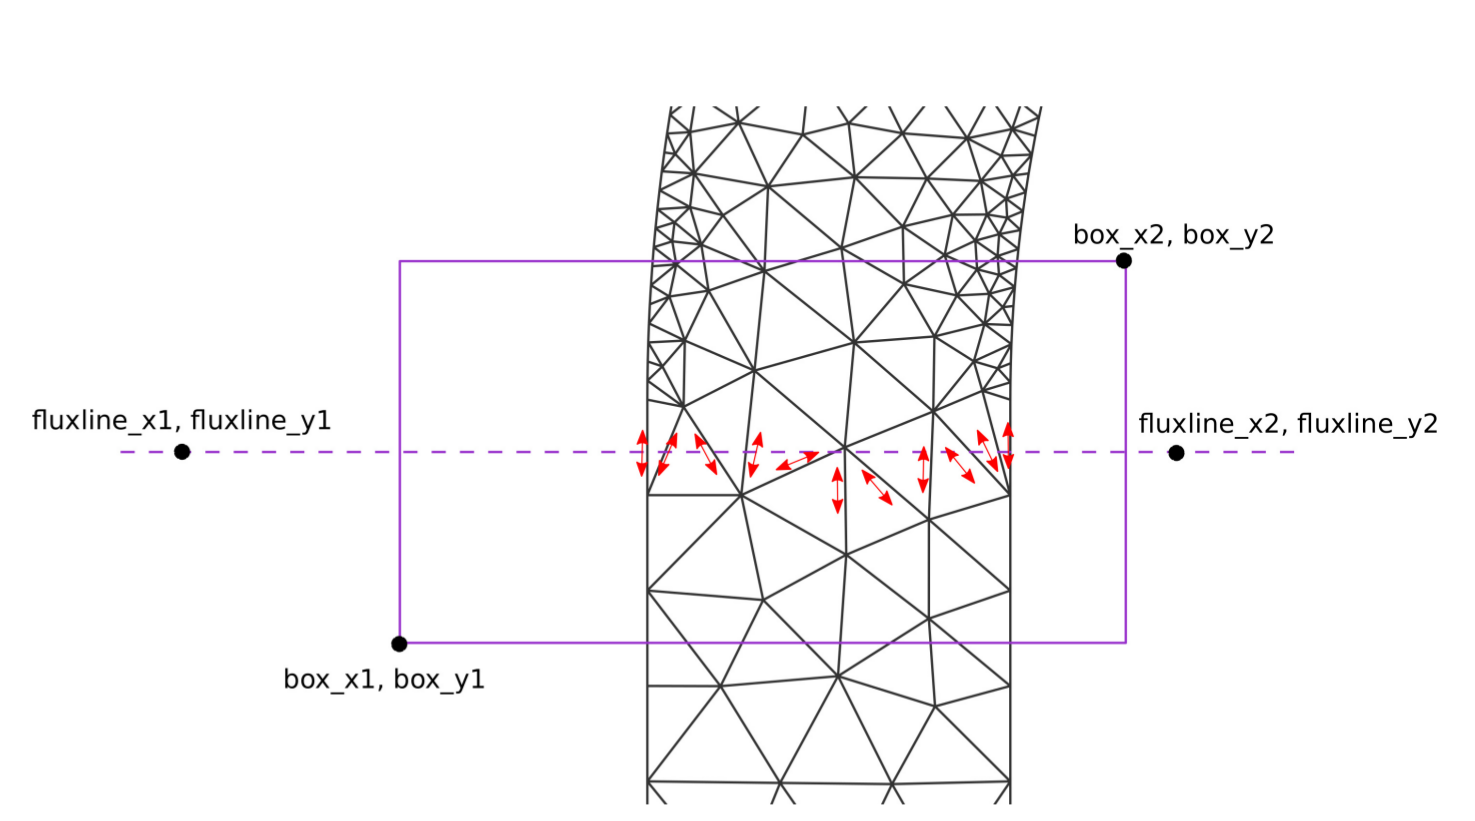
\includegraphics[scale=0.25,angle=0]{graphics/fluxline_example.png}
\caption{Description of a single fluxline and edge fluxes (red).}\label{fig:fluxline_example}
\end{center}
\end{figure}

Further details can be found in Stadler L. (2015) \textit{Calculating correct water and sediment fluxes in TELEMAC2D and SISYPHE}. Proceedings of the 22$^{nd}$
Telemac \& Mascaret User Club, STFC Daresbury Laboratory, UK, 13-16 October.

%\pagebreak
%-------------------------------------------------------------------------------
\section{Implement a new bedload transport formula}
%-------------------------------------------------------------------------------
To implement a new bedload transport formula, the keyword {\ttfamily BED-LOAD TRANSPORT FORMULA FOR ALL SANDS} must be set to {\ttfamily = 0}. The Fortran subroutine must be added into the Fortran file of \textsc{Telemac-2d} or \textsc{Telemac-3d}, keyword {\ttfamily FORTRAN FILE}.

The template subroutine is called \texttt{user\_bedload\_qb.f} and can be found in the folder \texttt{\$HOMETEL/sources/gaia}
\begin{lstlisting}[frame=trBL]
!               **************************
                SUBROUTINE USER_BEDLOAD_QB
!               **************************
     & (HN, U2D, V2D, THETAC, HOULE, HW, TW, THETAW,
     &  TOB,TOBW,TOBCW_MEAN,TOBCW_MAX, DCLA, DENS, GRAV, DSTAR, AC,
     &  XMVE, XMVS, TETAP, MU, NPOIN, QSC, QSS, CSTAEQ)
!
!***********************************************************************
! GAIA
!***********************************************************************
!
!>@brief Allows the user to code their own bedload transport
!!       formulation, best suited to their application.
!
!>@warning User subroutine; sand transport formula must be coded by the user
!>@todo Missing description of arguments
!
!~~~~~~~~~~~~~~~~~~~~~~~~~~~~~~~~~~~~~~~~~~~~~~~~~~~~~~~~~~~~~~~~~~~~~~~
!>@param[in]     HN
!>@param[in]     U2D
!>@param[in]     V2D
!>@param[in]     THETAC
!>@param[in]     HOULE
!>@param[in]     HW
!>@param[in]     TW
!>@param[in]     THETAW
!>@param[in,out] TOB
!>@param[in,out] TOBW
!>@param[in,out] TOBCW_MEAN
!>@param[in,out] TOBCW_MAX
!>@param[in]     DM
!>@param[in]     DENS
!>@param[in]     GRAV
!>@param[in]     DSTAR
!>@param[in]     AC
!>@param[in]     XMVE
!>@param[in]     XMVS
!>@param[in]     TETAP
!>@param[in]     MU
!>@param[in]     NPOIN
!>@param[in,out] QSC
!>@param[in,out] QSS
!>@param[in,out] CSTAEQ
!~~~~~~~~~~~~~~~~~~~~~~~~~~~~~~~~~~~~~~~~~~~~~~~~~~~~~~~~~~~~~~~~~~~~~~~
!
      USE INTERFACE_GAIA, EX_USER_BEDLOAD_QB => USER_BEDLOAD_QB
      USE BIEF
      USE DECLARATIONS_SPECIAL
      IMPLICIT NONE
!
!!-+-+-+-+-+-+-+-+-+-+-+-+-+-+-+-+-+-+-+-+-+-+-+-+-+-+-+-+-+-+-+-+-+-+-+
!
      TYPE(BIEF_OBJ),   INTENT(IN)    :: HN,U2D,V2D,THETAC
      TYPE(BIEF_OBJ),   INTENT(IN)    :: HW, TW, THETAW
      TYPE(BIEF_OBJ),   INTENT(IN)    :: TOB,TOBW,TOBCW_MEAN,TOBCW_MAX
      DOUBLE PRECISION, INTENT(IN)    :: DCLA, DENS, GRAV, DSTAR, AC
      DOUBLE PRECISION, INTENT(IN)    :: XMVE, XMVS
      TYPE(BIEF_OBJ),   INTENT(IN)    :: TETAP, MU
      TYPE(BIEF_OBJ),   INTENT(IN)    :: CSTAEQ
      INTEGER,          INTENT(IN)    :: NPOIN
      LOGICAL,          INTENT(IN)    :: HOULE
      TYPE(BIEF_OBJ),   INTENT(INOUT) :: QSC, QSS
!
!!-+-+-+-+-+-+-+-+-+-+-+-+-+-+-+-+-+-+-+-+-+-+-+-+-+-+-+-+-+-+-+-+-+-+-+
!
      INTEGER          :: I
!     DOUBLE PRECISION :: C1, C2, T
!
!======================================================================!
!======================================================================!
!                               PROGRAM                                !
!======================================================================!
!======================================================================!
!
!     EXAMPLE BY VAN RIJN
!
!     C1 = DENS * GRAV * DCLA
!     C2 = 0.053D0 * SQRT(DCLA**3*DENS*GRAV) * DSTAR**(-0.3D0)
!
      DO I = 1, NPOIN
!
!       TRANSPORT STAGE PARAMETER
!
!       IF(TETAP%R(I) .LE. AC) THEN
!         T = 0.D0
!       ELSE
!         T = (TETAP%R(I)-AC)/MAX(AC,1.D-06)
!       ENDIF
!
!       BEDLOAD TRANSPORT RATE
!
        QSC%R(I) = 0.D0 ! C2 * T**2.1D0
        QSS%R(I) = 0.D0
!
      ENDDO
!
!  FOLLOWING LINES NEED TO BE COMMENTED OUT
!
      WRITE(LU,53)

53    FORMAT(/,1X,'GAIA IS STOPPED : ',/
     &   ,1X,' SAND TRANSPORT MUST BE CALCULATED IN USER_BEDLOAD_QB')
      CALL PLANTE(1)
      STOP
!
!-----------------------------------------------------------------------
!
      RETURN
      END
\end{lstlisting}

%\pagebreak
%-------------------------------------------------------------------------------
%\section{Define a rigid bed}
%-------------------------------------------------------------------------------
%TODO
%\subsection{Data from selafin file}
%\subsection{Data coded by the user in the fortran file}

%\pagebreak
%-------------------------------------------------------------------------------
\section{Print a new output variable in the selafin file}
%-------------------------------------------------------------------------------
\begin{itemize}
\item Declare the {\ttfamily PRIVE} variable, for example as:

{\ttfamily USE DECLARATIONS\_GAIA, ONLY : PRIVE}

\item Use the following expression to include the variable you want to visualize:

{\ttfamily PRIVE\%ADR(N)\%P\%R(K) = [Here the variable you want to visualize]}, where {\ttfamily N} is the number of variables that you want to visualize and {\ttfamily K} is the number of nodes.

\item In the \gaia's steering file you can use the flags {\ttfamily'A'}, {\ttfamily'G'}, {\ttfamily'L'} or {\ttfamily'O'} to visualize the {\ttfamily PRIVE} variable, for example as:

{\ttfamily VARIABLES FOR GRAPHIC PRINTOUTS='U,V,S,H,B,Q,M,E,QSBL,TOB,MU,A'}
\end{itemize}

The default name {\ttfamily PRIVE 1} (for {\ttfamily N=1}) can be modified in the subroutine {\ttfamily nomvar\_gaia.f}.

\begin{lstlisting}[frame=trBL]
DO K=1, NPOIN
  PRIVE%ADR(1)%P%R(K) = [variable to visualize]
ENDDO
\end{lstlisting}

%\pagebreak
%-------------------------------------------------------------------------------
\section{Introduce a new keyword}
%-------------------------------------------------------------------------------
\begin{itemize}
\item In {\ttfamily declarations\_gaia.f} declare the variable to be called from a keyword e.g. {\ttfamily HMIN\_BEDLOAD}
\item In {\ttfamily lecdon\_gaia.f} declare .... {\ttfamily HMIN\_BEDLOAD=MOTREA(ADRESS(2,52))}
\item Declaration in the modified subroutine through {\ttfamily USE DECLARATIONS\_GAIA, ONLY : HMIN\_BEDLOAD}
\end{itemize}


%\pagebreak
%-------------------------------------------------------------------------------
% section to update
%\section{Read and use a variable from a selafin file}
%%-------------------------------------------------------------------------------
%Case of spatially distributed sediment zones
%
%\begin{itemize}
%\item Create the different zones with, e.g. BlueKenue
%\item Add in your steering file:
%  \begin{lstlisting}[frame=trBL]
%NUMBER OF PRIVATE ARRAYS = 1
%NAMES OF PRIVATE VARIABLES= 'ZONE                            '
%\end{lstlisting}
%(32 characters)%\textvisiblespace\textvisiblespace\textvisiblespace
%\item Modify the subroutine \texttt{init\_compo.f}, for example:
%\begin{lstlisting}[frame=trBL]
%      DO J=1,NPOIN
%      NCOUCHES(J)=1
%	  IF(PRIVE%ADR(1)%P%R(J).EQ.1.D0) THEN
%	  AVAIL(J,1,1)=1.D0
%	  AVAIL(J,1,2)=0.D0
%	  ELSEIF(PRIVE%ADR(1)%P%R(J).EQ.2.D0) THEN
%	  AVAIL(J,1,1)=0.D0
%	  AVAIL(J,1,2)=1.D0
%	  ELSE
%	  AVAIL(J,1,1)=0.5D0
%	  AVAIL(J,1,2)=0.5D0
%	  ENDIF
%      ENDDO
%\end{lstlisting}
%\end{itemize}


%\pagebreak
%-------------------------------------------------------------------------------
\section{Define the soil stratigraphy (\texttt{user\_bed\_init})}
%-------------------------------------------------------------------------------
In case of several layers with different sediment ratios, the subroutine \texttt{user\_bed\_init} must be used. \\
Here different layer thickness (\texttt{ESTRATUM}) and different mass ratios (\texttt{RATIO\_INIT}) for each sediment can be set.
For example for 2 layers and 4 sediments:
\begin{lstlisting}[frame=trBL]
      DO IPOIN=1,NPOIN
        ESTRATUM(1,IPOIN) = 0.12D0
        RATIO_INIT(1,1,IPOIN) = 0.5D0
        RATIO_INIT(2,1,IPOIN) = 0.5D0
        RATIO_INIT(3,1,IPOIN) = 0.D0
        RATIO_INIT(4,1,IPOIN) = 0.D0
        ESTRATUM(2,IPOIN) = 2.D0
        RATIO_INIT(1,2,IPOIN) = 0.D0
        RATIO_INIT(2,2,IPOIN) = 0.D0
        RATIO_INIT(3,2,IPOIN) = 0.5D0
        RATIO_INIT(4,2,IPOIN) = 0.5D0
      ENDDO
\end{lstlisting}

%\pagebreak
%-------------------------------------------------------------------------------
%\section{Suppress bed updating}
%-------------------------------------------------------------------------------
%Set \telkey{STATIONARY MODE = YES} (logical type, set to {\ttfamily = NO} by default)

%\pagebreak
%-------------------------------------------------------------------------------
\section{Using a non-declared variable in a \gaia{}'s subroutine}
%-------------------------------------------------------------------------------
If you want to use, for example, parameter \texttt{NPTFR} and the table \texttt{NBOR(NPTFR)} in a subroutine,
declare:

\texttt{USE DECLARATIONS\_GAIA, ONLY : NPTFR, MESH}

\texttt{INTEGER, POINTER :: NBOR(:)}

Then the following alias can be declared:

\texttt{NBOR=>MESH\%NBOR\%I}

%\pagebreak
%-------------------------------------------------------------------------------
\section{Deal with wetting and drying zones - use of
\telkey{MINIMAL VALUE OF THE WATER HEIGHT}}
%-------------------------------------------------------------------------------
At for example intertidal wetlands with flooding and drying or tidal areas, the
bottom friction could be very high when the water depth is very small, even for
small velocities, leading to high and unphysical erosion rates. To prevent that,
the keyword \telkey{MINIMAL VALUE OF THE WATER HEIGHT} can be used (real value,
by default equal to $1.0 \times 10^{-3}$m): the erosion rate will be set to zero
in nodes where h$<$h$_{min}$.
At the same time, in order to guarantee a balance between erosion and
deposition, even the deposition flux will be set to zero in the same nodes.\\
This keyword is activated when \telkey{TIDAL FLATS = YES} (default value). \\
In case of bedload, when using the keyword
\telkey{MINIMAL VALUE OF THE WATER HEIGHT},
the bedload fluxes (variable called QSC in \gaia) are also set to
zero if h$<$h$_{min}$. This is also applied when using total sediment transport
formulas (e.g. \telkey{BED-LOAD TRANSPORT FORMULA FOR ALL SANDS}
{\ttfamily= 30}). \\
Finally, the use of the keyword \telkey{MINIMAL VALUE OF THE WATER HEIGHT}
implies that the shear stress is set to zero to prevent unphysical values, if
h$<$h$_{min}$.
%@to do: describe how to use MINIMUM DEPTH FOR BEDLOAD
%\pagebreak
%-------------------------------------------------------------------------------
\section{Set a non-erodible bottom}
%-------------------------------------------------------------------------------
The non-erodible bottom (or rigid bed) can be set using the keyword \telkey{LAYERS INITIAL THICKNESS} which is equal to $100$~m by default, in case of a single layer. \\
For more complex set-up (e.g. rigid bed variable in space), the subroutine \texttt{user\_bed\_init} can be used. Here the variable \texttt{ESTRATUM} which states the thickness of the erodible bed, needs to be modify.
%\pagebreak
%-------------------------------------------------------------------------------
\section{Modify the bottom from the subroutine corfon}
%-----------------------------------------------------------------------------
For example, you want to set the bottom at node $325$ equal to $2.1$ m
\begin{itemize}
\item Sequential: \texttt{ZF\%R(325)=2.1D0}
\item Parallel: \texttt{ZF\%R(GLOBAL\_TO\_LOCAL\_POINT(325,MESH))=2.1D0}
\end{itemize}

If there are several nodes to be modified, use a loop.

{\footnotesize Thanks to JMH (post \#9747)}

%-------------------------------------------------------------------------------
\section{Dredge and dump activities}
%-------------------------------------------------------------------------------
When using the module \nestor (keyword: \telkey{NESTOR = YES}) to carry out dredge or dump activities, these files are used to
specify the action, location, geometry and the last status. The keywords identifying these files are:

\begin{enumerate}
\item  \telkey{NESTOR ACTION FILE}

\item  \telkey{NESTOR POLYGON FILE}

\item  \telkey{NESTOR SURFACE REFERENCE FILE}

\item  \telkey{NESTOR RESTART FILE}
\end{enumerate}

These files are described in detail in the \nestor User Manual.

%-------------------------------------------------------------------------------
\section{Morphological spin-up}
%-------------------------------------------------------------------------------
It is essential to start a morphological computation using fully developed hydrodynamic conditions. In an initial hydrodynamic computation, large velocities may occur, which lead to unphysical changes in the bed. There are two methods to achieve this:
\begin{enumerate}
\item Perform a separate hydrodynamic computation (without \gaia), for an initial spin up period. Use the results of this computation using the \telkey{PREVIOUS COMPUTATION FILE} in \telemac{2D} or \telemac{3D} as \textit{hotstart}.
\item Use the keyword  \telkey{SPINUP TIME FOR BED UPDATING} (real value equal to 0. by default). With this keyword, no bed level changes are taken into account during the first period of the calculation, specified with this keyword (in seconds). In this way, it is possible to perform the hydrodynamic spin-up in the morphological run, such that a second run is not needed.  In case of suspended sediment transport calculations, no bed changes due to erosion and deposition are taken into account in this period. However, the sediment concentration in the water column adapts to the hydrodynamic conditions including the erosion and deposition flux. In this way the suspended sediment concentration at the start of the morphological calculation can be in equilibrium with the hydrodynamic conditions, thus preventing rapid erosion at the initial period, typically found when starting with a water column without any suspended sediment. The keyword can thus be used for bedload, suspended load and both. An example of the use of this keyword can be found in the Yen test case.
\end{enumerate}

%-------------------------------------------------------------------------------
%\section{Set-up a graded sediment problem with only one layer}
%-----------------------------------------------------------------------------


%-------------------------------------------------------------------------------
\section{Continuing a computation}
%-------------------------------------------------------------------------------
\label{sec-restart}
Like \telemac{2D} or \telemac{3D}, \gaia enables the user to resume a
computation taking a time step
of a previous computation on the same mesh as initial state.

From v8p5, two methods are possible to continue a computation:
\begin{itemize}
\item continuing a computation using a restart file manually generated
by users from a previous computation (single solution up to v8p4),
\item continuing a computation using a restart file automatically generated
by \gaia (and \telemac{2D} or \telemac{3D}) (new method introduced in v8p5).
Advantages of this last approach are:
\begin{itemize}
  \item the result file only contains variables of interest for users
(and not variables necessary to restart, as for the first approach) which
allows files of smaller size.
In particular less variables are saved at every graphic printout
and no extra variables are needed for sediments of type CO,
  \item users do not have to think and select variables necessary for restart
as they are automatically chosen by the code during the first simulation,
  \item the restart is done without information losses for two reasons:
first, variables necessary for restart are grabbed from the restart file without
recomputing them by means of other variables;
second, the default option uses a double precision format to generate the
restart file.
The only drawback in this case is that this file is larger compared to the
single precision format.
\end{itemize}
\end{itemize}

The first approach is described here below.
By default, as for \telemac{2D} or \telemac{3D}, \gaia reads the last record of
the previous computation result file.
Using the keyword \telkey{RECORD NUMBER FOR RESTART} allows specifying
the number of the iteration to be read (default = -1 means the last record is
taken).
This keyword has been introduced in release v8.5
(before, it was only possible to continue a computation from the last record
of the \telkey{PREVIOUS SEDIMENTOLOGICAL COMPUTATION FILE}).

In this case, it is essential that the continuation file contains
all the information required by \gaia{}.
However, in some cases, the software is capable of recomputing some
variables from others provided.
If some variables are missing from the continuation file,
they are then fixed automatically at zero.

In order to use the continuation file, it is necessary to enter
two keywords in the steering file:

\begin{itemize}
\item The keyword \telkey{COMPUTATION CONTINUED} must have the value YES
(default value = NO),

\item The keyword \telkey{PREVIOUS SEDIMENTOLOGICAL COMPUTATION FILE} must
provide the name of the file that will supply the initial state.
\end{itemize}

N.B.: the mesh for which the results are computed must be exactly the same
as the one to be used in continuing the computation.

If necessary, the keyword
\telkey{PREVIOUS SEDIMENTOLOGICAL COMPUTATION FILE FORMAT}
can be used to select a specific format.
For example, in order to increase the accuracy of the initial state,
it is possible to use double precision SERAFIN format ('SERAFIND') or
MED format ('MED').
Obviously, this configuration is possible only if the previous computation
was correctly configured in terms of results file format.
\\

The second approach is described here below.
Resuming the computation usually leads to small differences in results
compared to the same calculation without interruption.
To correct this, the user has a specific recovery procedure
to improve the accuracy of calculations, using double precision format SERAFIN
files (or MED format) for the keyword \telkey{RESTART FILE FORMAT}
(default = SERAFIND):

\begin{itemize}
\item In the first computation, the keyword \telkey{RESTART MODE} is set to
YES (default = NO),
which generates a specific file containing the full information at one or a
few time step(s) of the simulation.
The name of this file is given by the keyword \telkey{RESTART FILE},

\item In the second computation, this specific file must be used as
\telkey{PREVIOUS SEDIMENTOLOGICAL COMPUTATION FILE} specifying the
\telkey{PREVIOUS SEDIMENTOLOGICAL COMPUTATION FILE FORMAT} is 'SERAFIND'
(SERAFIN double precision).
If the restart should be done from the last time step saved in the
\telkey{RESTART FILE}, the keyword \telkey{RECORD NUMBER FOR RESTART} is to be
let to default value (= -1), otherwise it should be changed.
\end{itemize}

In the first computation, there are 2 keywords which can enable to tune the
resuming of the computation:
\begin{itemize}
\item If wanting to generate a \telkey{RESTART FILE} at a specific number of
time step different from the last one, the keyword
\telkey{RECORD NUMBER IN RESTART FILE} is to be used
(default = -1 means the \telkey{RESTART FILE} is only written at the last
time step or periodically at the period \telkey{RESTART FILE PRINTOUT PERIOD}),
\item If wanting to generate a \telkey{RESTART FILE} periodically to secure a
file to resume computation in case of crash e.g., the keyword
\telkey{RESTART FILE PRINTOUT PERIOD} defines the printout period in number of
time steps.
Default = 0 means no periodic writing and variables are only written at the last
time step of the computation or at the time step number
\telkey{RECORD NUMBER IN RESTART FILE} if not equal to -1.
\end{itemize}

However, it has to be mentioned that even if it is not advisable, the creation
of specific restart file can be done not only SERAFIND format, but also with
any other available format in the TELEMAC system, especially in single
precision. In this case, the keyword \telkey{RESTART FILE FORMAT} (by default
set at 'SERAFIND') must be set to the proper value.
\\

When continuing a computation, it is necessary to specify the value of
the start time of the second computation via the keyword
\telkey{INITIAL TIME SET TO ZERO} in the \telemac{2D} or \telemac{3D} steering
file.

At the beginning of a simulation, the launcher creates a temporary directory
where all input files are copied.
This is also the case for the previous computation file which can be quite huge.
In this situation and to avoid copying too large a file,
it is recommended to extract the time step used for the continuation
(the only one used by \telemac{2D} or \telemac{3D} and \gaia{}).
\\

2 examples are provided to show how to handle this feature in the steering
files:
\begin{itemize}
\item mud\_conservation-t2d,
\item yen-t2d multi 1.
\end{itemize}

A triple coupling (\telemac{2D}, \gaia{} and \tomawac{}) is also provided
as an example to show how to handle this feature in the steering files.
It can be found in littoral-t2d-tom folder.
In particular for the \tomawac steering file:
\begin{itemize}
\item In the first computation, the name of the file to store wave information
to resume is given by the keyword \telkey{GLOBAL RESULT FILE} and its format
is given by the keyword \telkey{GLOBAL RESULT FILE FORMAT} (double precision
with SERAFIND or MED are welcome in order not to have loss of accuracy),

\item In the second computation, this specific file must be used as
\telkey{PREVIOUS COMPUTATION FILE} specifying the
\telkey{PREVIOUS COMPUTATION FILE FORMAT} is 'SERAFIND'
(SERAFIN double precision).
%No keyword \telkey{RECORD NUMBER FOR RESTART} in \tomawac at the moment
%If the restart should be done from the last time step saved in the
%\telkey{RESTART FILE}, the keyword \telkey{RECORD NUMBER FOR RESTART} is to be
%let to default value (= -1), otherwise it should be changed.
\end{itemize}

Currently, no loss of accuracy has been observed for some examples:
\begin{itemize}
\item bosse-t2d (FE+FV),
\item bump-t2d,
\item guenter-t2d,
\item hippodrome-t2d (all except  1COs\_vf),
\item littoral-t2d-tom,
\item mud\_conservation-t2d,
\item sliding-t2d,
\item yen-t2d (FE + FV + multi-layers).
\end{itemize}

Some differences have been observed when coupling \telemac{2D} and \gaia{} and
should be investigated:
\begin{itemize}
\item cvsm-t2d,
\item flume\_bc-t2d,
\item sandpit-t2d,
\item wilcock\_crowe-t2d,
\end{itemize}

There are also differences when coupling \telemac{3D} and \gaia.
Investigation would start by resolving such an issue (loss of accuracy)
when using \telemac{3D} only.
